%% Beamer Presentation using 16:9 aspect ratio (HDTV standard aspect ratio)
\documentclass[aspectratio=169]{beamer}

%% Metropolis or mtheme Theme
\usetheme{metropolis}

% Packages
\usepackage{fancyvrb}
\usepackage{graphicx}
\usepackage{listings}
\usepackage[]{hyperref, amsmath}
\usepackage{pgfplots}
\usepackage{appendixnumberbeamer}

% Provide an easy command for mono spaced font: \t{text}
\renewcommand{\t}[1]{\texttt{#1}}

% Provide an easy command for full screen graphics
\newcommand<>{\fullsizegraphic}[1]{
{
    \begin{frame}[plain]
        \begin{tikzpicture}[remember picture,overlay]
            \node[at=(current page.center)] {
                \includegraphics[width=\paperwidth]{#1}
            };
        \end{tikzpicture}
    \end{frame}
}
}
\newcommand<>{\fullsizegraphich}[1]{
{
    \begin{frame}[plain]
        \begin{tikzpicture}[remember picture,overlay]
            \node[at=(current page.center)] {
                \includegraphics[height=\paperheight]{#1}
            };
        \end{tikzpicture}
    \end{frame}
}
}

% Customize the Fancy Verbatim environment's default font and margins
\RecustomVerbatimEnvironment
{Verbatim}{Verbatim}
{formatcom=\scriptsize,xleftmargin=0.75ex}

% use filled blocks for default, alert and example blocks
\metroset{block=fill}

% Title format uses smallcaps
\metroset{titleformat=smallcaps}

% 42 Lines logo colors
\definecolor{blue}{RGB}{5,76,111}
\definecolor{lightblue}{RGB}{53,137,175}
\definecolor{grey}{RGB}{187,187,187}

% Adjust Metropolis theme to use 42 Lines colors
\setbeamercolor{alerted text}{fg=lightblue}
\setbeamercolor{example text}{fg=blue}
\setbeamercolor{palette primary}{bg=blue}

% Customization for code listings including font size, a background and margins
\lstset{
    basicstyle=\scriptsize\ttfamily,
    backgroundcolor=\color{normal text.bg!80!normal text.fg!50!normal text.bg},
    frame=single,
    framerule=0pt,
}

% 42 Lines logo in top right corner
\graphicspath{{../../42lines-template/}}
\titlegraphic{\hfill
\includegraphics[width=.15\textwidth]{42-LOGO}}

% Here ends the preamble

\usepgfplotslibrary{fillbetween}

\title{Observability Through the Lens of\\Metrics and Events}
%%\subtitle{Subtitle Foo on Bar}
\institute{42 Lines, Inc.}
\author{Jack Neely jjneely@42lines.net\\Breandan Dezendorf breandan@42lines.net}

\date{\today}

\begin{document}

\maketitle

\begin{frame}[fragile]
    \frametitle{What's a Metric?}

    Prometheus:
\begin{lstlisting}
# HELP http_requests_total total HTTP hits
# TYPE http_requests_total counter
http_requests_total 34877
# HELP node_load1 1m load average.
# TYPE node_load1 gauge
node_load1 1.35
\end{lstlisting}

    Graphite:
\begin{lstlisting}
servers.A.http.hits 34877 1234567890
servers.A.collectd.load.load.shortterm 1.35 1234567890
\end{lstlisting}

    OpenTSDB:
\begin{lstlisting}
put http.hits 1234567890 34877 host=A
put proc.loadavg.1min 1234567890 1.35 host=A
\end{lstlisting}
\end{frame}

\begin{frame}
    \frametitle{Time Series: \t{sum(rate(http\_requests\_total[5m]))}}
    \begin{center}

   \begin{tikzpicture}[]
        \begin{axis}[
            width=14cm,
            height=7cm,
            xlabel=Time,
            ylabel=Hits/s,
            xticklabel={$t_{\pgfmathprintnumber{\tick}}$},
            enlargelimits=false,
            ymin=40,
            ymax=110,
        ]
            \addplot+[no markers, thick] table[x expr=\coordindex, y index=0]{raw};
        \end{axis}
    \end{tikzpicture}
    \end{center}
\end{frame}

\begin{frame}
    \frametitle{Anomaly Detection: Moving Median 1 Hour Offset 10\% Range}
    \begin{center}

   \begin{tikzpicture}[]
        \begin{axis}[
            width=14cm,
            height=7cm,
            xlabel=Time,
            ylabel=Hits/s,
            xticklabel={$t_{\pgfmathprintnumber{\tick}}$},
            enlargelimits=false,
            ymin=40,
            ymax=110,
        ]
            \addplot+[no markers, color=blue, thick] table[x expr=\coordindex, y index=0]{raw};
            \addplot+[no markers, name path=high, color=grey] table[x expr=\coordindex, y index=0]{high};
            \addplot+[no markers, name path=low, color=grey] table[x expr=\coordindex, y index=0]{low};
            \addplot [grey] fill between [of=high and low];
        \end{axis}
    \end{tikzpicture}
    \end{center}
\end{frame}

\begin{frame}
    \frametitle{Basic Data Types}

    \textbf{Gauge:} Fluctuating Arbitrary Measurement
    \begin{itemize}
        \item Temperature
        \item Queue Size
        \item In Use File Descriptors
    \end{itemize}

    \textbf{Counter:} Continuously Incrementing (and Resetting)
    \begin{itemize}
        \item Number of Bytes / Packets on a Network Interface
        \item Events
    \end{itemize}

    \textbf{Stat:} Summary Statistics for a Distribution of Events
    \begin{itemize}
        \item Duration of Event
        \item Size of Event
    \end{itemize}
\end{frame}

\begin{frame}
    \frametitle{Gauges}

    \begin{theorem}[Nyquist–Shannon Sampling]
        If a function $x(t)$ contains no frequencies higher than $B$ hertz, it
        is completely determined by giving its ordinates at a series of points
        spaced $1 / 2B$ seconds apart.
    \end{theorem}

    \begin{center}
        \includegraphics[width=0.8\linewidth]{CPT-sound-nyquist-thereom-1.5percycle.png}
    \end{center}
\end{frame}

\begin{frame}
    \frametitle{Counters}

    \begin{definition}[Monotonic Function]
        A function is called monotonically increasing if for all $x$ and
        $y$ such that $x \leq y$ one has
        $f(x) \leq f(y)$, so $f$
        preserves the order.
    \end{definition}

    \begin{center}
    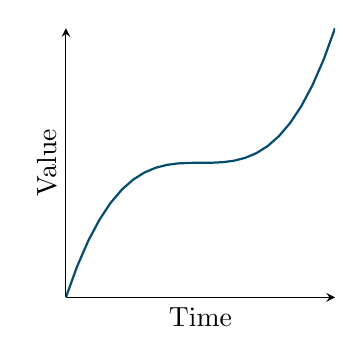
\begin{tikzpicture}[]
        \begin{axis}[
            width=5cm,
            height=5cm,
            xlabel=Time,
            ylabel=Value,
            enlargelimits=false,
            ticks=none,
            axis x line=bottom,
            axis y line=left,
        ]
            \addplot+[no marks, thick] {(x^3};
        \end{axis}
    \end{tikzpicture}
    \end{center}
\end{frame}

\begin{frame}
    \frametitle{Options for Metrics of Events and Cardinality}

    \begin{columns}
        \begin{column}{0.3\linewidth}
            StatsD -- Generate Summary Metrics Per Interval
            \begin{itemize}
                \item Count
                \item Sum
                \item Min
                \item Max
                \item Percentiles
            \end{itemize}
        \end{column}
        \begin{column}{0.7\linewidth}
            \begin{center}
            \begin{tikzpicture}
                \begin{axis}[
                    ylabel=Frequency,
                    xlabel=Cummlative Histogram,
                    ybar interval,
                    grid=none,
                    xtick align=inside,
                    x tick label as interval=false,
                    xtick=,% reset from ybar interval
                    %xticklabel={$(\pgfmathprintnumber\tick - \pgfmathprintnumber\nexttick)$},
                ]

                    \addplot+[hist={cumulative,data=x,data max=120,bins=12}]file {rand_hist.dat};
                \end{axis}
            \end{tikzpicture}
            \end{center}
        \end{column}
    \end{columns}
\end{frame}

\begin{frame}
    \frametitle{Data Alignment and Reporting}

    \begin{center}
        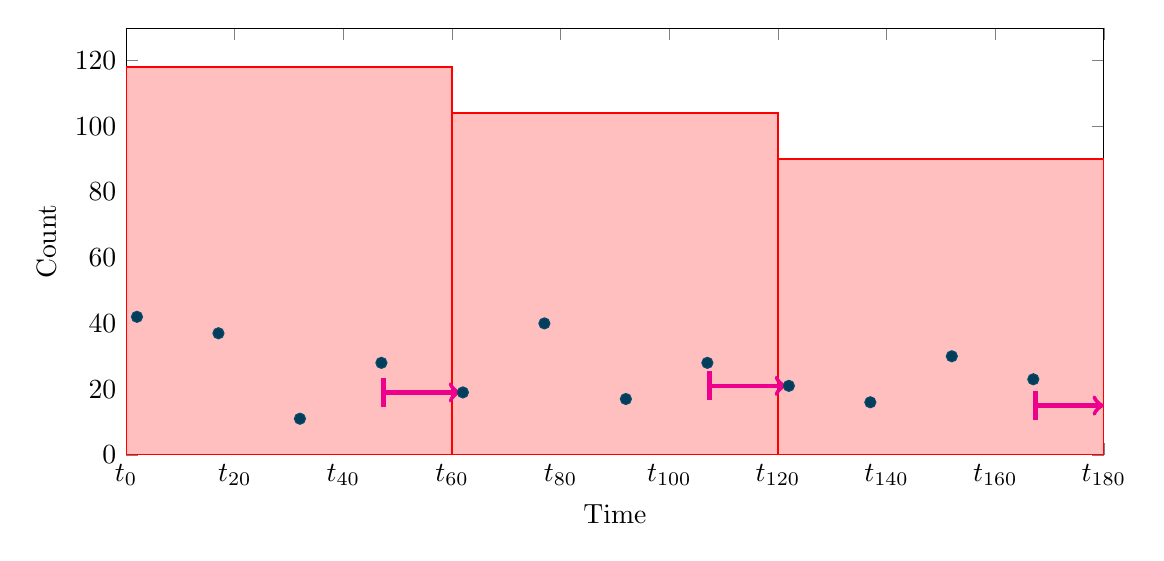
\begin{tikzpicture}[]
            \begin{axis}[
                width=14cm,
                height=7cm,
                xlabel=Time,
                ylabel=Count,
                xticklabel={$t_{\pgfmathprintnumber{\tick}}$},
                xmin=0, ymin=0, xmax=180
            ]
                \addplot+[only marks] coordinates {
                    (2, 42)  % 118
                    (17, 37)
                    (32, 11)
                    (47, 28)
                    (62, 19) % 104
                    (77, 40)
                    (92, 17)
                    (107, 28)
                    (122, 21) % 67+N
                    (137, 16)
                    (152, 30)
                    (167, 23)
                };
                \addplot+[ybar interval,fill=pink,mark=none] coordinates {
                    (0, 118)
                    (60, 104)
                    (120, 90)
                    (180, 0) % ybar interval extra coord
                };
                \draw[ultra thick,magenta,|->,shorten >=1pt] (47,19) to (62,19);
                \draw[ultra thick,magenta,|->,shorten >=1pt] (107,21) to (122,21);
                \draw[ultra thick,magenta,|->] (167,15) to (180,15);
            \end{axis}
        \end{tikzpicture}
    \end{center}
\end{frame}

\begin{frame}[fragile]
    \frametitle{What's an Event?}
An event is simply a record of a something happening at a given time.
\\
Standard apache access log:
\begin{lstlisting}
127.0.0.1 - - [12/Sep/2019:31:32:000 -0000] "GET / HTTP/1.0" 200 2216
\end{lstlisting}
\\
JSONLines formatted example of the same event:
\begin{lstlisting}
{
  "timestamp":"2019-09-12T19:31:32.000Z",
  "http_status_code": 200,
  "request": "GET / HTTP/1.0",
  "http_size_bytes": 2216
}
\end{lstlisting}
\end{frame}

\begin{frame}[fragile]
    \frametitle{Event Schema}

    Schema on read Schema on write
    Splunk is on-read, Elasticsearch/Solr/Graylog are on Write

\end{frame}

\begin{frame}[fragile]
    \frametitle{Schema On Write: Elasticsearch/Lucene}
    Keeps costs in control
    Allows for column-stride reads
    Makes filters very fast
\end{frame}
\begin{frame}[fragile]
    \frametitle{Common Data Types}
    Lucene isn't just for text anymore!
    \begin{lstlisting}
    - keyword vs text
    - float
    - geopoint
    - geoshape
    \end{lstlisting}
\end{frame}

\begin{frame}
    \frametitle{How Do Events Compare to Metrics?}
    \begin{itemize}
      \item 100x the cost to run an event system than a metrics system
      \item Free-form data blobs are costly to parse, store, retrieve and search
      \item Costly in memory, disk, CPU, and network I/O
      \item Guidelines for organization of data is hand wavy at best
    \end{itemize}
\end{frame}

\begin{frame}
    \frametitle{Why Use Events At All?}
    \begin{itemize}
      \item Able to investigate data after the fact
      \item Cardinality isn't nearly as expensive as it is for metrics
      \item Events often have more than one metric associated
    \end{itemize}
\end{frame}

\begin{frame}
    \frametitle{Example: latency per endpoint}
    \begin{itemize}
      \item Metric for latency per endpoint is cheap and fast. loading 30 days takes 1s
      \item Event calculation for the same takes 90s if it complets at all
      \item Now, get latency per endpoint per country
      \item With metrics, you can't if you didn't know you wanted it
    \end{itemize}
\end{frame}



\begin{frame}
    \frametitle{Guidelines for Using Metrics}

    \begin{itemize}
        \item Count Performance
        \item Key Health Indicators
        \item Limited Debugging with Feature Flags
        \item Make a Plan for Cardinality
        \item Look for Histogram Support
        \item Have a ``kit'' for SOA Metrics
    \end{itemize}
\end{frame}

\begin{frame}
    \frametitle{Guidelines for Using Logs and Events}
    Event size matters
    Parsing steps matter
    Storage costs and speed matter
    Sampling
\end{frame}

\begin{frame}
    \frametitle{Use Consistent Hashing to Coorelate Events}
    Generate a hash at the loadbalancer or entrypoint
    Save them as keywords in the event
    Allows for "find all events matching uuid=foo"
\end{frame}

\begin{frame}
    \frametitle{Use Consistent Hashing to Coorelate Events}
    Murmur3 hashing is fast, memory safe and has a very consistent spread
    logstash code example
\end{frame}

\begin{frame}
    \frametitle{sampling based on the consistent hash score}
    Once you have a murmur3 hash (which is a 32bit value), you can simply divide by maxint to get a score
    eg: a hash value of (X) is the numeric (Y) and when divided out is 0.3421
    Drop anything below a given value
    Send to a longer term index
\end{frame}

\begin{frame}
    \frametitle{save sampling rate to re-hyrdrate data with later}
    If you know your sampling score, save it to the event record
    Also save a scaledCount score, which is the inverse of the sampling rate. (eg, a sampling 1/10 events means the scaledCount value is 10/1)
    When graphing, simply run a sum aggregation on scaledCount rather than a simple count
\end{frame}


    




\begin{frame}[standout]
    Thank You!
\end{frame}

\appendix

\end{document}
